\chapter{SLG/Al$_{2}$O$_{3}$基板におけるコバルトインターカレーション}

本章ではグラフェンにおけるスピン軌道相互作用の増大を目指し,グラフェン/サファイア基板におけるコバルトのインターカレーションの研究についてまとめる.
まず化学蒸着(CVD:chemical vapor deposition)法によってSLGを作成した結果及びコバルトの蒸着について述べる.その後作成したSLGの質を評価した結果をまとめる.最後にコバルトインターカレーションについての結果を述べる.第\ref{chap:intro}章の\pageref{subsec:graphene}ページの\ref{subsec:graphene}で述べたように本研究ではCVD法を用いてグラフェンを作成した.まずこれについて述べる.

\section{CVD法によるSLGの作成及びコバルトのEB蒸着}
\subsection{CVD法によるSLG成長}
ここでは本研究で用いたSLGの作成について述べる.まず(0001)面Al$_{2}$O$_{3}$基板をダイアモンドペンを用いて$1\rm\ cm \times 1\rm\ cm$に切り分けた.この$1\rm\ cm \times 1\rm\ cm$のAl$_{2}$O$_{3}$基板の表面の有機物をクリーニングするために大気中で900$\rm\ C^{\circ}$を保ち6時間アニールをした.CVDを行うガラス管はFig.\ref{fig:CVD}のような形状である.

\begin{figure}[htbp]
 \begin{center}
  
\includegraphics[width=100mm]{images/CVD.eps}
 \end{center}
 \caption{CVD法の概略図.緑の球が炭素,オレンジの球が水素,紫の玉がアルゴンを示している.}
 \label{fig:CVD}
\end{figure}

このガラス管の中にAl$_{2}$O$_{3}$基板を用意し,内部を$1.6\times10^{-5}\rm\ Pa$の真空にする.そこで内部の空間及び基板表面の有機物を取り除くために300$\rm\ C^{\circ}$で1時間アニールした.その後菅内部の温度を1時間ほどかけて1000$\rm\ C^{\circ}$にし,安定に1000$\rm\ C^{\circ}$になった時にメタノールガスを流す.そこで真空をひくポンプ(ターボ分子ポンプ)から切り離しCVD用のポンプ(ロータリーポンプ)だけで菅の真空を引き始める.これにより内部圧力が上がり$2.6\times10^{2}\rm\ Pa$ほどで定常状態になる.内部圧力の増加によりCVDに必要な化学反応が始まる.その後4時間1000$\rm\ C^{\circ}$を保持しCVDを行なった.4時間経過した直後にCVDによるグラフェンの成長を止めるためターボ分子ポンプによる真空引きを開始し,同時にドライヤーを用いて急冷した.この急冷の温度勾配が重要である.急冷によって基板における化学反応の停止及び炭素の結合を促すと考えられている.そのためできるだけ素早く行なった.CVDが終わった直後の菅内部の圧力は$2.0\times10^{2}\rm\ Pa$となっていた.
CVDが終わったあとにこの後に述べるラマン分光法によりグラフェンが実際に成長しているかどうかを確認し,その質を評価した.その後グラフェンの成長が確認できた試料にコバルトを蒸着した.

\subsection{SLG/Al$_{2}$O$_{3}$におけるコバルト蒸着}

SLG上にコバルトを蒸着するためにEB(electron beam)蒸着法を用いた.EB蒸着法とは電子線を用いて金属ターゲットを加熱することでそれを蒸発させて基板に金属薄膜を形成する方法である.金属薄膜を作成する方法は他にも存在するがスパッタリング法のような蒸着する金属分子のエネルギーが高い方法はグラフェンを傷つけてしまい欠陥が生まれてしまう.それを避けるためにEB蒸着法を選択した.
蒸着チャンバーにSLG/Al$_{2}$O$_{3}$試料を入れSLGのクリーニングのため600$\rm\ C^{\circ}$にして20 min加熱した.加熱することによりSLGに付着した有機物が蒸発しチャンバー内部の圧力が増加する.その圧力が$10^{-6}\rm\ Pa$程度になった時にクリーニングを終えた.その後コバルトのレートが$0.05\rm\ \AA/sec$で一定になるようにフィラメント電流を24 mAにし,定常状態になってから蒸着を開始しコバルトをSLG/Al$_{2}$O$_{3}$上に2原子層蒸着した.

\subsection{Co/SLG/Al$_{2}$O$_{3}$のアニールによるインターカレーション}
インターカレーションは試料を加熱することにより分子が他の分子組織に入り込む現象である.そのため他のグループを参考にし真空中でアニールをすることによりコバルトをSLG/Al$_{2}$O$_{3}$界面にインターカレートさせようと考えた.
真空中で基板を加熱することによりインターカレーションを目指した.実際には600$\rm\ C^{\circ}$から800$\rm\ C^{\circ}$までアニール温度を変えてインターカレーションが起こる温度を探索した.温度はパイロメータで測定した温度に対応している.
\begin{table}[htbp]
 \caption{インターカレーションアニールの条件.}
 \begin{center}
  \begin{tabular}{ccc}\toprule
  基板加熱装置の温度計 (C$^{\circ}$)	&	パイロメータの温度表示	(C$^{\circ}$)	&	真空度 (Pa)	\\	\hline 
	562		&	392 			&	$1.8\times10^{-7}$\\
	620   &   565      &  $3.0\times10^{-7}$  \\
	768  &	712			&	$2.1\times10^{-6}$	\\
	893  &   820  &    $5.2\times10^{-6}$     
						\\	\bottomrule
  \end{tabular}
 \end{center}
 \label{tb:ICcond}
\end{table}

基板加熱装置にも温度計が付いているがその温度計は基板ホルダーの温度を示しているため,実際の基板の温度とは乖離している.その温度とアニールした時のチャンバー内の圧力は表\ref{tb:ICcond}にまとめた.

\section{ラマン分光法によるSLGの評価}
\subsection{ラマン分光法について}
次にAl$_{2}$O$_{3}$上にグラフェンが成長しているのかを確認するために行ったラマン分光測定の原理及びその結果について述べる.

ラマン分光とは光の非弾性散乱である.光の散乱の前後でエネルギーが変化しないものをレイリー散乱という.レイリー散乱では光の電場が分子の中で振動する双極子モーメントが発生し,その双極子モーメントの振動によって電場が新たに生成され散乱が起きる.一方その双極子モーメントが分子振動を引き起こすことがある.これは電子-格子相互作用を介し双極子モーメントのエネルギーの一部が分子振動に受け渡される.つまりこの時,双極子モーメントの振動によって発生する光のエネルギーは分子振動のエネルギー分だけ減少している.これがラマン効果である.格子振動は量子化されその振動数を$\omega$とするとラマン散乱光のエネルギーは入射した光のエネルギーから$\hbar\omega$を差し引いたエネルギーを持つ.この散乱光をCCDカメラなどで測定すると入射光のエネルギーから$\hbar\omega$だけずれたエネルギー(ラマンシフト)において強い散乱光強度を得られる.これをラマンスペクトルと呼び,分光された各波長の情報を波数(cm$^{2}$)に換算しFig.\ref{fig:ramanshift}のようなスペクトルにする.

\begin{figure}[htbp]
\centerline{
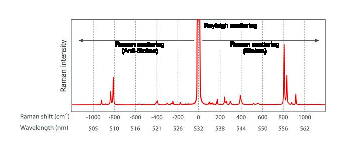
\includegraphics[width=12cm]{images/ramanshift.eps}
}
\caption{ラマンシフトの例.
}
\label{fig:ramanshift} 
\end{figure}
レイリー散乱は弾性散乱のためエネルギー損失がなく散乱しエネルギーシフトは起きない.ラマンシフトがレイリー散乱のスペクトルから長波長側及び短波長側に観測されていることがわかるが,これは双極子モーメント振動から分子振動にエネルギーを与える(長波長側)だけでなく双極子モーメントが分子振動からエネルギーをもらう(短波長側)の散乱過程も可能なためである.これはそれぞれストークス線,及びアンチストークス線と呼ばれる.実際は強度の強いストークス線を用いて解析される.
格子振動数$\omega$は分子の種類や結合状態によって異なるため,ラマンスペクトルを測定することで分子の状態や構造に関する情報を手に入れることができる.横軸は分子の振動情報(結合状態や電子状態),縦軸の比は活性の強さを反映している.




ラマン散乱効果では入射光の波長は関係ないが,入射光のエネルギーがラマンスペクトルを得たい物質の吸収エネルギーに一致する場合はラマン強度は著しく強くなる.このとき共鳴ラマン分光という.第\ref{chap:intro}章における\pageref{sec:graphene}で述べたようにグラフェンは可視光付近の光に対して光吸収を伴うため,可視光に対してグラフェンは常に共鳴ラマン分光となる.この効果のためにグラフェンは一層($0.335\rm\ nm$)であってもラマン分光が観測できる.またFig.\ref{fig:ramanshift}からもわかるように散乱光のほとんどはレイリー散乱による光であり.レマン散乱光はレイリー散乱の$10^{-6}$程度であるため実際の光源は強度の強いレーザー光を用いた.

\subsection{ラマンスペクトルの測定結果}
次にAl$_{2}$O$_{3}$基板上にCVD法によってSLGが成長できたかを確認するためにラマン分光測定を行なった結果を述べる.比較対象として転写法を用いてSiO$_{2}$基板上に作成したSLGのラマンスペクトルを載せた.その結果がFig.\ref{fig:raman_init}である.
\begin{figure}[htbp]
\centerline{
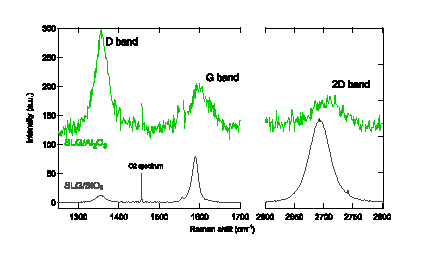
\includegraphics[width=12cm]{images/raman_init.eps}
}
\caption{SLG/SiO$_{2}$およびSLG/Al$_{2}$O$_{3}$のラマンスペクトル.
}
\label{fig:raman_init} 
\end{figure}

SiO$_{2}$上のグラフェンのラマン散乱光は増強されることが知られグラフェンの一般的なラマンシフトを示すのに適している.Figure.\ref{fig:raman_init}の灰色の線で示したSLG/SiO$_{2}$のスペクトルのようにグラフェンに特有なバンドは3つある.一つは$1580\rm\ cm^{-1}$付近にあるGバンドである.これはsp$^{2}$混成軌道に共通されるバンドである.また$2700\rm\ cm^{-1}$付近にある2Dバンドもグラフェン特有である.これは散乱時のグラフェン内のディラックコーンの電子の励起における二重共鳴ラマン効果により生じる.$1350\rm\ cm^{-1$付近に存在するDバンドはグラフェンの欠陥により生じるバンドである.DとGバンドの比はグラフェンの結晶性にほぼ比例すると知られている.また一般的に2DバンドとGバンドの比はグラフェンの層数に比例している.層数が増加するほどGバンドに対する2Dバンドの強度は小さくなる.1層の時は2Dバンドの方が大きく2層以上になるとGバンドの方が大きくなる.

SLG/SiO$_{2}$と比較してSLG/Al$_{2}$O$_{3}$のDバンド/Gバンドの比は大きくなっている.これは酸化物上におけるSLGの成長が難しいことを示している.しかしGバンド及び2Dバンドの存在からAl$_{2}$O$_{3}$上にSLGを成長させることに成功したことがわかる.2DバンドがGバンドより小さいのはグラフェンの層数が2層である可能性,もしくはキャリアドープの効果が考えられる\textcolor{blue}{[ドープの論文]}.実際,グラフェンが成長した表面に二層目のグラフェンが成長することは難しくCVDが進行しないことが考えられるため,この結果からAl$_{2}$O$_{3}$との結合によりグラフェンの電子状態がSiO$_{2}$上に成長している時とは異なっていることが予想される.
ノイズが大きく見えるのはSLG/SiO$_{2}$のラマンスペクトル強度が増強されているためにノイズが潰れていて,対照的にSLG/Al$_{2}$O$_{3}$のノイズが大きいように見える.

Al$_{2}$O$_{3}$上にSLGが成長しているのが確認できた.次にこの試料を用いてコバルトインターカレーションの実現を目指した.


\section{コバルトインターカレーションの評価}
コバルトがSLG/Al$_{2}$O$_{3}$界面にインターカレートすることを観測するために選択した方法がXPS測定の角度依存性を用いた方法である.XPSとはX線光電子分光(X-ray Photoelectron Spectroscopy)法の略語であり,その名の通りX線を用いて原子軌道の電子を光電子として励起させ,その光電子のエネルギーから原子の種類や状態を測定する方法である.その概略図をFig.\ref{fig:XPS_concept}に描いた.

\begin{figure}[htbp]
\centerline{
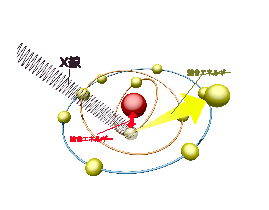
\includegraphics[width=12cm]{images/XPS_concept.eps}
}
\caption{XPS測定の概要図.X線が原子に入射した時その入射エネルギー$h_{\nu}$が電子の結合エネルギー$E_{\rm B}$以上だと電子を結合状態からはじき出し光電子として放出する.その光電子の持っているエネルギー$E_{\rm k}$から原子の電子状態や構造が解析できる.
}
\label{fig:XPS_concept} 
\end{figure}

原子にエネルギー$h_{\rm\nu}$を持ったX線を照射すると原子内部の結合エネルギー$E_{\rm B}$で核に束縛された電子が励起され,運動エネルギー$E_{\rm K}$を持った光電子として飛び出す.その光電子の$E_{\rm K}$は物質の仕事関数$\phi$を用いて

\begin{eqnarray}
E_{\rm K} = h_{\rm\nu} - E_{\rm B} -\phi
\label{eq:XPS1}
\end{eqnarray}
と表せる.ここから式を変形すると
\begin{eqnarray}
E_{\rm B} = h_{\rm\nu} - E_{\rm K} -\phi
\label{eq:XPS2}
\end{eqnarray}
となる.このとき照射したX線のエネルギーは自身で決定し仕事関数は求めることができるので既知である.つまり光電子の運動エネルギーを測定することで光電子を束縛していた結合エネルギーの値を定量することができる.結合エネルギーは物質と軌道の組み合わせに対して一対一対応しているため,結合エネルギーを定量することでX線を照射した表面に存在する物質を調べることができる.
またX線の侵入長が数nmであることからXPSは表面敏感な測定である.このことを利用しXPS測定の角度依存性を用いることによって表面付近の元素分布の深さ分解を定量することができる.
\begin{figure}[htbp]
\centerline{
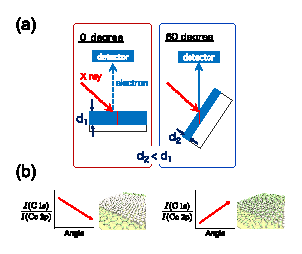
\includegraphics[width=10cm]{images/XPSAng_concept.eps}
}
\caption{XPS測定の角度分解の概要図.(a)X線の入射角が0度のときと60度のときを比較すると,60度のときの方がX線の侵入深さが浅くなっている.このように試料のX線に対する傾きを変化させることによって角度分解を行なった.(b)炭素とコバルトの強度比$I(\rm C\ 1s)/I(\rm Co\ 2p)$の角度に対する振る舞いによって再表面にある物質を同定づることが可能である.
}
\label{fig:XPSAng_concept} 
\end{figure}

Figure.\ref{fig:XPSAng_concept}(a)のようにX線の入射角を深くするとX線によって励起される原子の深さが浅くなる.つまり角度をつければつけるほどより表面敏感になる.これを用いることによって深さ方向の物質分布を定量することができる.XPSの角度分解を利用することによって,コバルトがインターカレートしていない場合Co/SLGの順番なので角度を浅くしていくとコバルトの強度が相対的に増加していくはずである.逆にコバルトがSLGの下に潜った場合,SLG/Coなので角度を増加していくと炭素の強度が増加していく.Fig.\ref{fig:XPSAng_concept}(b)に示すように,コバルトの強度を$I(\rm Co\ 2p)$,炭素の強度を$I(\rm C\ 1s)$と表すと,角度に対しての振る舞いが逆になるはずである.
実際の実験の流れはコバルトをSLG/Al$_{2}$O$_{3}$上に蒸着した試料をアニールし,その試料のXSP測定の角度分解を行い,その後再度アニール温度を変えて試料を焼くことを繰り返した.この工程は全て真空中で行なった.ただしアニールは$10^{-6}\rm\ Pa$,XPS測定は$10^{-7}\rm\ Pa$台の下で行なった.

\subsection{XPS測定}
では実際のXPS測定の結果を述べる.
XPS測定で得られる生に得られるデータはある運動エネルギーを持った光電子がどれだけ検出されたかというものである.スペクトルは横軸が光電子の運動エネルギー(eV)であり縦軸がその運動エネルギーを持った光電子の検出されたカウント数(counts/sec)である.しかし実際に物質の種類などを同定するために必要な値は運動エネルギーではなく結合エネルギーである.そこで式\ref{eq:XPS2}を用いて運動エネルギーを結合エネルギーに変換しなくてはならない.本研究ではXPSにおけるX線源としてMgK\alpha を用いているためX線のエネルギーは1253.6 eVである.エミッションカレントは10.0 mAに一定しにて電圧は100 kVとした.パスエナジーは50に設定した.あと必要な値は仕事関数$\phi$である.ここで今回のような絶縁体(半導体などの導電性の低い材料)を取り扱う場合,実際問題としてXPS測定は中性のX線を照射し負に帯電している電子を放出させているため試料が正に帯電してしまう.この帯電(チャージアップ)のため仕事関数とは別に光電子に対するエネルギー障壁が増加する.この仕事関数とチャージアップの影響を含めたエネルギー障壁を$\Phi$とすると式\ref{eq:XPS2}における$\phi$を$\Phi$に書き換えられる.この分まで補正するために通常は試料の基板に含まれる元素(試料の変化に伴って状態が変化しないものを選択する)のスペクトルピークで補正をかける.今回の研究では基板に含まれるAlを基準とした.例えばAl2pのピークだとわかるスペクトルのピーク位置が86 eVだとする.式\ref{eq:XPS2}を考えて,まずX線のエネルギーから運動エネルギーである86 eVを引くと,$E_{\rm B}+\Phi = 1253.6-86=1167.6\rm\ eV$となる.実際のAl2pの結合エネルギーは$74.7\rm\ eV$なので,$\Phi = 1167.6 - 74.7 = 1092.9\rm\ eV$となる.つまり得られた生データの横軸である光電子の運動エネルギー$E_{\rm K}$から$E_{\rm B}$を求めるためには

\begin{eqnarray}
E_{\rm B} = 1253.6 - E_{\rm K} -1092.9 = 160.7 -E_{\rm K}
\label{eq:XPS3}
\end{eqnarray}
という変換をすれば結合エネルギーを得られる.ただし物質の仕事関数は一定であるがチャージアップは測定するたびに装置の状況(真空度など)や測定環境(温度や湿度)によって変化するため,アニールした後などXPS測定チャンバーから移動するたびに補正項$\Phi$を計算した.以上の補正をして得られた600$\rm\ C^{\circ}$でアニールしたCo/SLG/Al$_{2}$O$_{3}$についてのXPSスペクトルがFig.\ref{fig:600aneal_1st_0deg}である.
\begin{figure}[htbp]
\centerline{
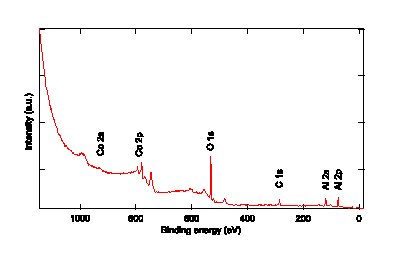
\includegraphics[width=12cm]{images/600aneal_1st_0deg.eps}
}
\caption{600$\rm\ C^{\circ}$でアニールしたCo/SLG/Al$_{2}$O$_{3}$のXPSスペクトル.コバルト,炭素及びAl$_{2}$O$_{3}$のアルミニウムと酸素のピークが見える.他のピークが見られないことから不純物のコンタミが少ないと考えられる.
}
\label{fig:600aneal_1st_0deg} 
\end{figure}

これはワイドスキャンと呼ばれ,表面に存在する元素を網羅的に確認するために行った.しかしこのワイドスキャン時は大雑把に把握するのが目的のためステップ数を荒く設定した.ワイドスキャン後に詳細に定量したい元素のピーク付近のナロースキャンを行なった.XPS測定時の設定を参考のために表\ref{tb:XPScondition}にまとめた.
\begin{table}[htbp]
 \caption{XPS測定時の条件設定}
 \begin{center}
  \begin{tabular}{cccc}\toprule
  	スキャン	&	ステップ幅(eV)	&	パスエナジー		&	積算回数	\\	\hline
	ワイド(全体を網羅的)	&	1.007		&	100	&	10				\\
	Al2p&	0.061		&	50		&	70
	\\
	C1s&  0.061  &    50  & 400
	\\
	Co2p& 0.061  &   50   &   100
						\\	\bottomrule
  \end{tabular}
 \end{center}
 \label{tb:XPScondition}
\end{table}

ただしステップ数は測定点間隔を表す.パスエナジーとは,運動エネルギー$E_{\rm\ B}$からパスエナジーだけずれたエネルギーを持つ光電子を$E_{\rm\ B}$になるように加速・減速させてXPS装置の検出器に入れる.つまりパスエナジーが大きいほど検出強度(検出される光電子数)は大きくなるがその分誤差は大きくなる.また積算回数は600$\rm\ C^{\circ}$でアニールした際の値であり,測定ごとに解析に十分なスペクトル形状となるような値を選んだ.(Coがインターカレートした際には炭素がコバルトの上にあるためコバルトの強度が弱くなるのでその分コバルトの積算回数を大きくした.)コバルトとグラフェン由来の炭素及びAl$_{2}$O$_{3}$基板のアルミニウムと酸素のピークが見える.ここからは他の物質のコンタミは確認できなかった.

次にFig.\ref{fig:600aneal_1st_0deg}のナロースキャンの結果をFig.\ref{fig:600aneal_1st_0deg_narrow}に示す.

\begin{figure}[htbp]
\centerline{
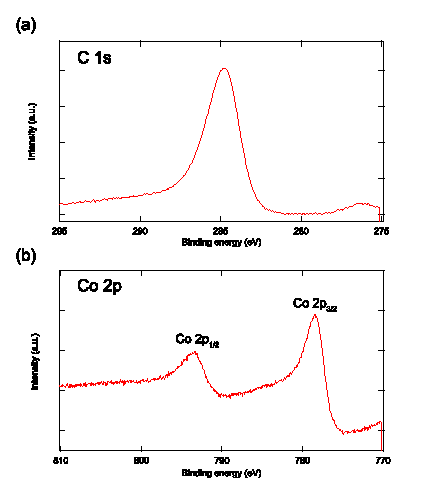
\includegraphics[width=10cm]{images/600aneal_1st_0deg_narrow.eps}
}
\caption{600$\rm\ C^{\circ}$でアニールしたCo/SLG/Al$_{2}$O$_{3}$のC1s(a)及びCo2p(b)のピーク.(b)コバルトの2p軌道はスピン軌道相互作用によって2p$_{1/2}$と2p$_{3/2}$の2準位に分裂している.
}
\label{fig:600aneal_1st_0deg_narrow} 
\end{figure}

コバルトの2p軌道はスピン軌道相互作用により縮退がとけ2p$_{1/2}$と2p$_{3/2}$の二つのピークが存在する.以上の結果は試料に対しX線は垂直(0度)に照射している.インターカレートが起きている確認するために炭素とコバルトの強度比$I(\rm C\ 1s)/I(\rm Co\ 2p)$を求める.この強度として本研究ではスペクトルの面積を用いた.コバルトは2p$_{3/2}$のピーク面積をその強度として用いた.このときこの600$\rm\ C^{\circ}$でアニールしたCo/SLG/Al$_{2}$O$_{3}$の0度の時の炭素とコバルトの強度比は$I(\rm C\ 1s)/I(\rm Co\ 2p) = 3.35$であった.
0度の時と同様の測定をX線の試料に対する照射角度を60度にして行なった.そのときの炭素とコバルトの強度比は$I(\rm C\ 1s)/I(\rm Co\ 2p) = 2.74$であった.角度を増加させると炭素に対するコバルトの強度が増加しているこの結果は表面にコバルトが多く存在していることを示している.つまり600度アニールではコバルトのインターカレーションは起きていないことがわかる.

次に同じ試料をアニールのチャンバーに移し700度のアニールをして再度XPS測定を行なった.その結果のワイドスキャン及びC1s,Co2pのスペクトルをFig.\ref{fig:700aneal_1st}に示す.

\begin{figure}[htbp]
\centerline{
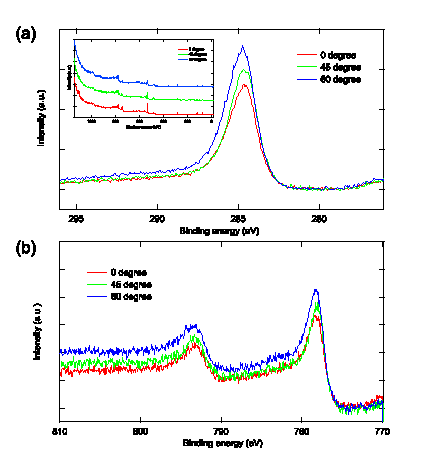
\includegraphics[width=10cm]{images/700aneal_1st.eps}
}
\caption{700$\rm\ C^{\circ}$でアニールしたCo/SLG/Al$_{2}$O$_{3}$のC1s(a)及びCo2p(b)のピーク.インセットはワイドスキャンを示している.
}
\label{fig:700aneal_1st} 
\end{figure}

この結果からピーク面積を求めてその炭素とコバルトの強度比は$I(\rm C\ 1s)/I(\rm Co\ 2p)$を定量した.その結果をFig.\ref{fig:rate_comparison}に示す.

\begin{figure}[htbp]
\centerline{
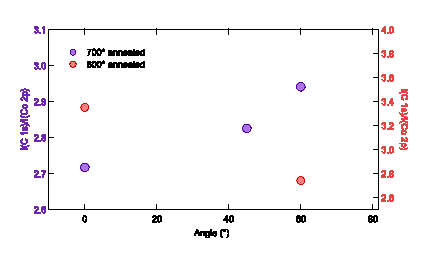
\includegraphics[width=10cm]{images/rate_comarison.eps}
}
\caption{600$\rm\ C^{\circ}$及び700$\rm\ C^{\circ}$でアニールしたCo/SLG/Al$_{2}$O$_{3}$の炭素とコバルトの強度比$I(\rm C\ 1s)/I(\rm Co\ 2p)$の角度依存性.
}
\label{fig:rate_comparison} 
\end{figure}

XPS測定はX線の照射角度が大きくなるほど,より表面敏感な測定になるためFig.\ref{fig:rate_comparison}の600$\rm\ C^{\circ}$アニールの結果のように$I(\rm C\ 1s)/I(\rm Co\ 2p)$の比が角度に対して小さくなっていくのは表面にコバルトが存在していることを表している.対してFig.\ref{fig:rate_comparison}における700$\rm\ C^{\circ}$アニールの結果のように角度を大きくしていくほど$I(\rm C\ 1s)/I(\rm Co\ 2p)$の比が増加してくのは,表面にコバルトより炭素が多くあることを示している.つまりCo/SLG/Al$_{2}$O$_{3}$を700$\rm\ C^{\circ}$でアニールすることによってコバルトがSLG/Al$_{2}$O$_{3}$界面にインターカレートしたことを示唆している.

コバルトのインターカレーションをさらに確認するために試料を大気中に取り出した後の試料を再度XPS測定した.というのも,もしコバルトがSLG/Al$_{2}$O$_{3}$界面にインターカレートしていた場合SLGが酸化防止膜として働き,界面に存在するコバルトが参加しないことが予想される.一方コバルトがSLGの上に存在していた場合はコバルトが酸化されるはずである.酸化コバルトにおける2p軌道の電子状態は酸素との結合によりコバルトにおけるものから変化しているため,XPS測定で判別できる.もっともわかりやすい変化は,コバルトの2p$_{1/2}$ピークと2p$_{3/2}$ピークの差$\Delta_{\rm Co2p}$の変化である.コバルトは$\Delta_{\rm Co2p} = 15.05\rm\ eV$であるが,酸化コバルトCoOでは$\Delta_{\rm Co2p} = 10.5\rm\ eV$となる.そこで700$\rm\ C^{\circ}$アニールをした後大気暴露した場合コバルトが酸化するかを確認するために,SLG/Al$_{2}$O$_{3}$上にコバルトを蒸着した試料を700$\rm\ C^{\circ}$アニールしたものとアニールをしなかったものを大気にさらしその後真空中に戻しXPS測定行ない,コバルトの2p軌道の電子状態を観測した.その結果がFig.\ref{fig:atom_comparison}である.

\begin{figure}[htbp]
\centerline{
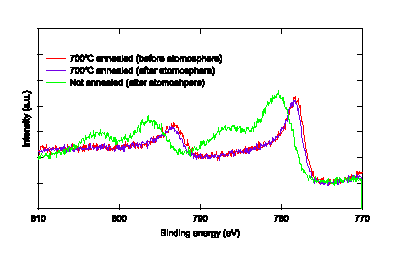
\includegraphics[width=12cm]{images/atom_comparison.eps}
}
\caption{Co/SLG/Al$_{2}$O$_{3}$のCo2pピーク.赤のスペクトルは700$\rm\ C^{\circ}$アニールして大気に出さずXPS測定をしたもの.紫のスペクトルは700$\rm\ C^{\circ}$アニールした後大輝暴露し,再度真空中に戻しXPS測定をした試料.緑のスペクトルはコバルトをSLG/Al$_{2}$O$_{3}$上に蒸着した後アニールをせず大気暴露し,その後真空に戻しXPS測定した試料.
}
\label{fig:atom_comparison} 
\end{figure}

比較対象として700$C^{\circ}$アニールした後に大気暴露せずにXPS測定した結果(赤のスペクトル,Fig.\ref{fig:700aneal_1st}(b)における0degの結果と同様.)も載せてある.この結果を見ると700$C^{\circ}$アニールした試料は大気暴露後も大気に出す前のスペクトルとほとんど変化していない.一方アニールをせずに大気暴露した試料はスペクトル形状が変化していて,$\Delta_{\rm Co2p}$も増加している.$\Delta_{\rm Co2p}$をそれぞれ表\ref{tb:atom_comparison}にまとめた.

\begin{table}[htbp]
 \caption{Fig.\ref{fig:atom_comparison}における$\Delta_{\rm Co2p}$}
 \begin{center}
  \begin{tabular}{cc}\toprule
  	試料	&	$\Delta_{\rm Co2p}$	eV	\\	
  	\hline
	700$C^{\circ}$ annealed	(before atomosphere)&	15.08						\\
	700$C^{\circ}$ annealed	(after atomosphere)&	15.20		
	\\
	Not annealed (after atomosphere)&  15.56  
						\\	\bottomrule
  \end{tabular}
 \end{center}
 \label{tb:atom_comparison}
\end{table}




さらにアニールをしていない試料は2p$_{1/2}$ピークと2p$_{3/2}$ピークそれぞれの高エネルギー側にサテライトピークが存在している.これらからアニールをせずに大気暴露した試料はコバルトが酸化していると言える.これらの結果からアニールをした試料のコバルトだけが大気暴露しても酸化しないことが分かった.これはアニールしたことによってコバルトがSLGの下に入り込みSLGの酸化防止膜の効果によって酸化が防がれていることを示唆している.

これらの試料についてラマン分光測定をした.次にその結果について述べる.

\subsection{ラマン分光測定}

Co/SLG/Al$_{2}$O$_{3}$をアニールすることでSLGの電子状態が変化していないかを確認するためにCo/SLG/Al$_{2}$O$_{3}$を700 C$^{\circ}$したものとアニールをしていないもののラマン分光測定を行なった.ただしラマン分光測定は待機中で行なった.その結果がFig.\ref{fig:raman_comparison}である.

\begin{figure}[htbp]
\centerline{
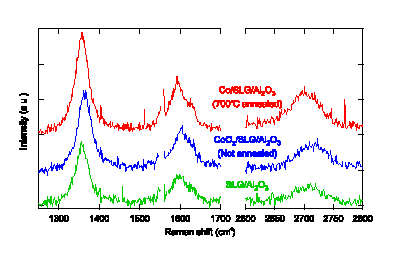
\includegraphics[width=12cm]{images/raman_comparison.eps}
}
\caption{SLG/Al$_{2}$O$_{3}$およびCo/SLG/Al$_{2}$O$_{3}$のラマンスペクトル.緑のスペクトルがコバルトを蒸着する前のSLG/Al$_{2}$,赤のスペクトルがCo/SLG/Al$_{2}$を700 C$^{\circ}$アニールしたもの,青のスペクトルがアニールをしていないCo/SLG/Al$_{2}$のラマンスペクトルを示している.
}
\label{fig:raman_comparison} 
\end{figure}

この結果からSLG由来のバンドがシフトしていることがわかる.しかしこの電子状態の変化がコバルトのインターカレートによるものなのか他の要因なのかは,より詳細な解析が必要である.


\subsection{AFM測定による評価}
コバルトがインターカレートしたCo/SLG/Al$_{2}$O$_{3}$としたいない試料の表面はコバルトがあるかないかで異なるはずである.この予想のもとAFM測定によって表面形状を観察した.その結果をFig.\ref{fig:AFM_SLG}である.
\begin{figure}[htbp]
\centerline{
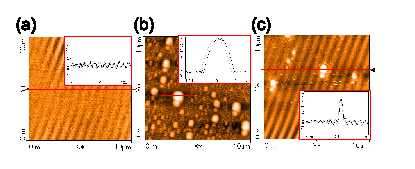
\includegraphics[width=12cm]{images/AFM_SLG.eps}
}
\caption{SLG/Al$_{2}$O$_{3}$およびCo/SLG/Al$_{2}$O$_{3}$のAFM像.一辺10 $\rm\mu m$の走査範囲である.(a)SLG/Al$_{2}$O$_{3}$,(b)アニールをしていないCo/SLG/Al$_{2}$O$_{3}$,(c)700 C$^{\circ}$でアニールをしたCo/SLG/Al$_{2}$O$_{3}$の像.インセットはそれぞれ赤い線で切り取った表面形状を表している.}
\label{fig:AFM_SLG} 
\end{figure}

Fig.\ref{fig:AFM_SLG}の(a)では見えない粒子が(b)では見えている.これはコバルトがアイランド状に凝集しているものだと考えられる.コバルトはSLG上ではその濡れ性のために,ごく薄い領域では表面エエルギーを低くするために薄膜にはならずアイランド上にまとまる.一方アニールした試料AFM像(c)ではその粒子が少なっている.これはアニールしたことによってコバルトがSLGの下にもぐったことを示唆している.少しSLG上に残っているコバルトのために,700 C$^{\circ}$アニールしたCo/SLG/Al$_{2}$O$_{3}$を大気暴露したあとXPS測定をした際に酸化コバルトの影響が見えたと予想される.(表\ref{tb:atom_comparison}で700$C^{\circ}$ annealed (after atomosphere)も多少の変化が見られる.)

section{まとめ}

